\documentclass[twoside,twocolumn,a4paper,10pt]{article}

\usepackage{blindtext} % Package to generate dummy text throughout this template 

\usepackage{mathptmx}
%\usepackage[sc]{mathpazo} % Use the Palatino font
\usepackage[T1]{fontenc} % Use 8-bit encoding that has 256 glyphs
\linespread{1.05} % Line spacing - Palatino needs more space between lines
\usepackage{microtype} % Slightly tweak font spacing for aesthetics

\usepackage[english]{babel} % Language hyphenation and typographical rules

\usepackage[hmarginratio=1:1,left=15mm,right=15mm,top=32mm,columnsep=20pt]{geometry} % Document margins
\usepackage[hang, small,labelfont=bf,up,textfont=it,up]{caption} % Custom captions under/above floats in tables or figures
\usepackage{booktabs} % Horizontal rules in tables

\usepackage{lettrine} % The lettrine is the first enlarged letter at the beginning of the text

\usepackage{enumitem} % Customized lists
\setlist[itemize]{noitemsep} % Make itemize lists more compact

\usepackage{abstract} % Allows abstract customization
\renewcommand{\abstractnamefont}{\normalfont\bfseries} % Set the "Abstract" text to bold
\renewcommand{\abstracttextfont}{\normalfont\small\itshape} % Set the abstract itself to small italic text

\usepackage{titlesec} % Allows customization of titles
\renewcommand\thesection{\Roman{section}} % Roman numerals for the sections
\renewcommand\thesubsection{\roman{subsection}} % roman numerals for subsections
\titleformat{\section}[block]{\large\scshape\centering}{\thesection.}{1em}{} % Change the look of the section titles
\titleformat{\subsection}[block]{\large}{\thesubsection.}{1em}{} % Change the look of the section titles

\usepackage{fancyhdr} % Headers and footers
\pagestyle{fancy} % All pages have headers and footers
\fancyhead{} % Blank out the default header
\fancyfoot{} % Blank out the default footer
\fancyfoot[RO,LE]{\thepage} % Custom footer text

\usepackage{titling} % Customizing the title section

\usepackage{booktabs}       % pour de jolis tableaux
%\usepackage{fancyhdr}       % pour des entêtes et pieds de pages améliorés.
\usepackage{makeidx}        % requis pour faire les index
\usepackage{amsmath}
\usepackage{amssymb}
\usepackage{mathtools}
\usepackage{amsfonts}
\usepackage{amssymb}
\usepackage{color}
\usepackage{array}
\usepackage{graphicx}
\usepackage{animate}
\usepackage{caption} 
\usepackage{hyperref}
\usepackage{algorithm}
\usepackage{algorithmic}
\usepackage{subcaption}
\usepackage{times}
\usepackage{tabularx}
\usepackage{authblk}
\usepackage{multirow}
\usepackage{array}

\providecommand{\keywords}[1]{\textbf{\textit{keywords :}} #1}
\renewcommand{\thesubsection}{\Alph{subsection}}

     % Ce fichier contient tous les packages nécessaires à la compilation


\title{\textbf{Automatic clustering for of MRI images, application on perfusion MRI of brain.}}

\author{%
  \textsc{Philippe Chuzel, Ali Mansour}\\%
		\normalsize Lab-STIC\\%
		\normalsize ENSTA Bretagne\\%
		\normalsize Brest, France\\%
\and 
	\textsc{J. Gentric}\\%, J. Ognard, L. Bressollette
		\normalsize Lab GETBO\\%
		\normalsize Brest university hospital Cavale Blanche\\%
		\normalsize Brest, France\\%
  }
  
\date{}

%----------------------------------------------------------------------------------------

%\author[1]{P. Chuzel}
%\author[1]{A. Mansour}
%\author[2]{J. Ognard}
%\author[2,3]{J. Gentric}
%\author[4]{D. Hamad}
%\author[5]{N. Betrouni}
%\author[2]{L. Bressollette}
%\begin{small}
%\affil[1]{ENSTA Bretagne, 2 rue F. Verny, 29200 Brest, France.}
%\affil[2]{Brest university hospital Cavale Blanche, Boulevard T. Prigent, 29200 Brest, France.}
%\affil[3]{Lab GETBO , equipe 3878, Brest Cavale Blanche, Boulevard T. Prigent, 29200 Brest, France.}
%\affil[4]{Universit\'e du Littoral-C\^ote-d'Opale ULCO, 50 Rue F. Buisson, 62100 Calais, France.}
%\affil[5]{INSERM Lille, 1 Avenue O. Lambret, 59260 Lille, France.}
%\end{small}
%\date{}

%----------------------------------------------------------------------------------------
%\textsc{Philippe Chuzel} \\[1ex]
%\normalsize ENSTA Bretagne \\
%\normalsize \href{mailto:philippe.chuzel@ensta-bretagne.org}{philippe.chuzel@ensta-bretagne.org} 
%\and % Uncomment if 2 authors are required, duplicate these 4 lines if more
%\textsc{Ali Mansour} \\[1ex] % Second author's name
%\normalsize ENSTA Bretagne \\ % Second author's institution
%\normalsize \href{mailto:ali.mansour@ensta-bretagne.fr}{ali.mansour@ensta-bretagne.fr} % Second author's email address
%\and % Uncomment if 2 authors are required, duplicate these 4 lines if more
%\textsc{Denis Hamad} \\[1ex] % Second author's name
%\normalsize INSERM Lille \\ % Second author's institution
%\normalsize \href{mailto:denis.hamad@gmail.com}{denis.hamad@gmail.com} % Second author's email address
%\and % Uncomment if 2 authors are required, duplicate these 4 lines if more
%\textsc{Julien Ognard} \\[1ex] % Second author's name
%\normalsize CHRU Brest \\ % Second author's institution
%\normalsize \href{mailto:julien.ognard@chu-brest.fr}{julien.ognard@chu-brest.fr} % Second author's email address
%\and % Uncomment if 2 authors are required, duplicate these 4 lines if more
%\textsc{Nacim Betrouni} \\[1ex] % Second author's name
%\normalsize INSERM Lille \\ % Second author's institution
%\normalsize \href{mailto:nacim.betrouni@inserm.fr}{nacim.betrouni@inserm.fr} % Second author's email address
%\and % Uncomment if 2 authors are required, duplicate these 4 lines if more
%\textsc{Jean-Christophe Gentric} \\[1ex] % Second author's name
%\normalsize CHRU Brest \\ % Second author's institution
%\normalsize \href{mailto:jean-christophe.gentric@chu-brest.fr}{jean-christophe.gentric@chu-brest.fr} % Second author's email address

\begin{document}
  \setlength{\absparindent}{1cm}
  \setlength{\absparsep}{1cm}
  \setlength{\absleftindent}{0pt}
  \setlength{\absrightindent}{0pt}


%----------------------------------------------------------------------------------------
%	Abstract
%----------------------------------------------------------------------------------------

\maketitle
    \begin{abstract}
      \textbf{Many studies have been made in order to propose automatic diagnostic in medical fields. This paper proposes a new approach to deal with the problem of spectral clustering for signal extracted from brain MRI images. The tool-chain developed during this study can be easily implemented for the extraction and the analysis of information from perfusion MRI. We propose a reliable program which can easily isolate healthy from any pathological tissues. Experimental results are shown and discussed.}
    \end{abstract}
    \textit{\keywords{Spectral clustering, Signal and Image processing, Automatic segmentation, MRI}}
\medskip


%----------------------------------------------------------------------------------------
%	ARTICLE CONTENTS
%----------------------------------------------------------------------------------------

\section{Introduction}

Physicians use different sources of images in order to make a diagnostic. In the last two decades, many studies have been made in order to automatise the identification and the characterisation of disease by extracting relevant information from those sources of images like the MRI, the Elastography or the Echography, in order to propose help to diagnostic \cite{tartare2014contribution}, \cite{schmitt2011characterization}, \cite{schmitt2013shear}, \cite{ophir1991elastography}.

In \cite{tartare2014contribution}, a new methodology was proposed in order to realise an automatic segmentation of tumour tissues for prostate cancer. Our objective is to generalise and modify the previously proposed method to improve the segmentation of MRI images to diagnose brain pathologies.

Our project focuses on the perfusion MRI by using a spectral clustering algorithm. Physicians use perfusion MRI in order to check the variation of pixel intensity of the MRI image and identify abnormal behaviour. To apply similar methodology, we have to develop a unsupervised classification approach. The main issue is that many classification algorithms like the k-means are not suitable for signal classification. The main purpose of spectral clustering is to firstly estimate the similarity among signals and, build a similarity matrix and work on the eigenvector and eigenvalue of this matrix in order to perform a classification. Spectral clustering algorithms are the most adapted for the data we are dealing with.

This study is the result of a collaboration among four institutes: ENSTA Bretagne, Brest Hospital university Research Center (CHRU), INSERM of Lille and ULCO.

We apply our approach on a perfusion MRI database of twelve patients showing different pathologies in the brain in order to apply our algorithm.Those MRI have been provided by the Brest CHRU. An example of MRI images obtained can be seen in the figure \ref{fig:diffusion}. For each pixel, a variation of the intensity on the different MRI images can be observe.

\begin{figure}
\centering
\begin{subfigure}[t]{0.22\textwidth}
\centering
    \vspace{0.00\textheight}
    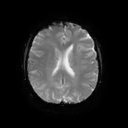
\includegraphics[scale=0.9,angle=0]{Im1.png}
    \caption{MRI without contrast product}
    \label{fig:without} 
\end{subfigure}
\begin{subfigure}[t]{0.22\textwidth}
\centering
    \vspace{0.00\textheight}
    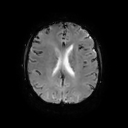
\includegraphics[scale=0.9,angle=0]{Im7.png}
    \caption{beginning of the diffusion}
    \label{fig:First} 
\end{subfigure}
\begin{subfigure}[t]{0.22\textwidth}
\centering
    \vspace{0.00\textheight}
    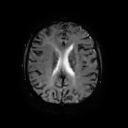
\includegraphics[scale=0.9,angle=0]{Im8.png}
    \caption{Peak of diffusion}
    \label{fig:Second} 
\end{subfigure}
\begin{subfigure}[t]{0.22\textwidth}
\centering
    \vspace{0.00\textheight}
    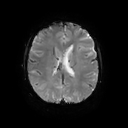
\includegraphics[scale=0.9,angle=0]{Im13.png}
    \caption{end of the diffusion}
    \label{fig:Last} 
\end{subfigure}
    \caption{Diffusion of the contrast product on the MRI.}
    \label{fig:diffusion} 
\end{figure}

%At the beginning, we wanted to apply those results for detection and the characterisation of the thrombus and the deep venous thrombosis. Many options are studied in order to achieve this goal like the use of Elastography and echography \cite{schmitt2011characterization}, \cite{schmitt2013shear}, \cite{ophir1991elastography}.We wanted to apply this methodology which use the MRI images as a new source of information on the clot. Nevertheless, we arrived quickly to those results:
%
%\begin{itemize}
%
%\item The MRI signature of the clot is highly dependent on its age, its composition and surrounding tissues.
%
%\item The position of the clot is not fixed. The clot can be naturally dissolved. 
%
%\item The composition of the clot can be known only through an extraction from the patient, which is not always possible. 
%
%\end{itemize}




%------------------------------------------------

\section{Methodology}

Our database consists of perfusion MRI. During a perfusion MRI, the patient is injected by a contrast product, the gadolinium chelates. It's well known and considered that normal and pathological tissues have different way and speed absorption of the contrast product. Pathological tissues have a very specific behaviour which can be detected by our algorithm.

Figure \ref{fig:Processing_toolchain} our proposed bloc diagram.

\begin{figure*}[h]
\centering
    \includegraphics[width=\textwidth,height=5cm]{Processing_toolchain.png}
    \caption{The proposed processing tool-chain.}
    \label{fig:Processing_toolchain}
\end{figure*}



In our database and for each patient, 26 sets of 40 images have been generated, each set is corresponding to a slice of the brain. The size of each image is 128*128 pixels. Each set is used in order to retrieve the variation of pixel intensity of the slice MRI during the diffusion of contrast product.

For each slice, we generate a 128*128*40 tensor. For each pixel, we extracted a signal of 40 samples which correspond to the variation of this pixel intensity in the 40 images of 128*128 pixels. Figure \ref{fig:CourbeExample} shows the generated signals using this protocol.

\begin{figure}
\centering
    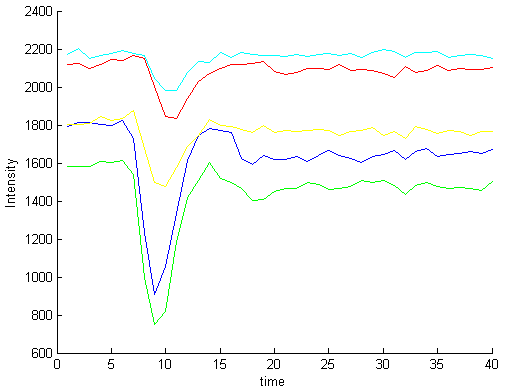
\includegraphics[scale=0.5,angle=0]{CourbeExample.png}
    \caption{Examples of signals extracted from the MRI.}
    \label{fig:CourbeExample}
\end{figure}

Figure \ref{fig:CourbeExample} shows that we obtain a hypo-signal during the diffusion of the contrast product until the intensity of the pixel come back to its original value. Our algorithm method afterwards selects a specific region of interest (ROI) on a slice and then apply a spectral clustering algorithm on those selected signals in order to cluster the different tissues of the area.






%------------------------------------------------

\section{Spectral Clustering Algorithms}


In the litterature, many references about the spectral clustering can be found \cite{von2007tutorial}, \cite{mouysset2010contributions}. However, we will here focus on the Jordan and Weiss spectral clustering algorithm JWSC \cite{von2007tutorial} because is very adapted to the unsupervised classification and it has provided the most satisfying results on the data we are dealing with. At the beginning, our algorithm builds a graph with its similarity matrix in order to evaluate the resemblance of the signal between them. In a second time, we will apply JWSC algorithm in order to cluster the signal thanks to the information extract from the similarity matrix.


\subsection{Definition of the similarity matrix.}

In order to have an algorithm independent from the processed data, we considered only full connected graph because it can estimate the resemblance of each sample with no a priori information. In a full connected graph, all the nodes are connected to each other.

In order to build the similarity matrix $W$, two different options have been studied :

\begin{itemize}

\item First option uses a sparse representation based on building a $L_1$ graph. The main idea consists on rebuild each point $X_i$ with all the other samples, according to a $L_1$ minimisation problem \cite{yan2009semi}.

\item Second option consists on defining $W$ as:
\begin{equation}
w_{ij} = \frac{\|X_i-X_j\|}{2\sigma_i\sigma_j}
\end{equation}
$\sigma_i$ is the coefficient of dispersion in the data around a point $X_i$ , \cite{tartare2014contribution}, \cite{mouysset2010contributions}. During the study, we found that the optimum value of $\sigma_i$ was the distance to the $7^{th}$ closest neighbour of the point $X_i$.

\end{itemize}

During the realization of the tool-chain, the first option was implemented but didn't give satisfaction. However, the second one on the contrary gave better results. The tool-chain use the second method for the construction of the graph and the matrix $W$.


\subsection{Spectral clustering algorithm.}

Many algorithms can be used for the spectral clustering, and some of them have been implemented during this project, \cite{von2007tutorial}, \cite{ng2002spectral},  \cite{shi2000normalized}. We give here details on the Jordan and Weiss algorithm.

To implement the JWSC algorithm, we have firstly to define the Laplacian matrix $L$ of the matrix $W$. The Laplacian is defined by :

\begin{equation}
L = I-D^{-1/2}WD^{-1/2}
\end{equation}

where $D$ is the degree matrix defined by its coefficient $d_{ii} = \sum_j w_{ij}$, a diagonal matrix ad $I$ is the identity matrix.

The processing tool-chain estimates the eigenvector associated to the smallest eigenvalues of $L$, normalizes each of them and realizes a classification using the k-means algorithm. The main steps of the JWSC algorithm are resumed in the algorithm \ref{alg:algorithm1}:

\begin{algorithm}
  \caption{Normalized spectral clustering, Jordan and Weiss }
  
  \textbf{Inputs}% Inputs section
  \begin{algorithmic}[1]
    \STATE Initiate the similarity matrix $W$
    \STATE Define the number of class $N$
  \end{algorithmic}
  \bigskip

  \textbf{Output}% Output section
  \begin{algorithmic}[1]
    \STATE The Cluster table $truth\_table$.
  \end{algorithmic}
  \bigskip
  
  \textbf{Algorithm}
  \begin{algorithmic}[1]
		\STATE Define the symmetric normalized Laplacian $L$ of $W$.
     	\STATE Create a matrix $VectP$ which contains the N eigenvectors associated with the N smallest eigenvalues.
     	\STATE Normalize all the line of $VectP$
     	\STATE Apply the k-means on $VectP$ with $N$ class and put the result in $truth\_table$.	
  \RETURN $truth\_table$
  \end{algorithmic}
  \label{alg:algorithm1}
\end{algorithm}

The main outcome of the algorithm is a truth table clustering all pixels in the ROI.


%------------------------------------------------

\section{Results}

Figure \ref{fig:Clean} represents a MRI of a patient with brain tumour. Figure \ref{fig:CleanGray} shows the area of pathological tissue.

\begin{figure}
\centering
    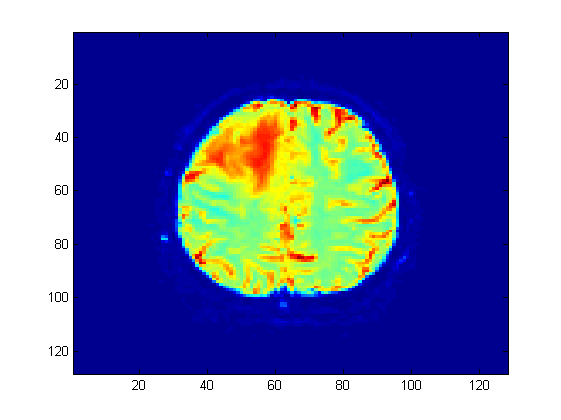
\includegraphics[scale=0.5,angle=0]{Imageclean.png}
    \caption{First image of the MRI with false color.}
    \label{fig:Clean}
\end{figure}

\begin{figure}
\centering
    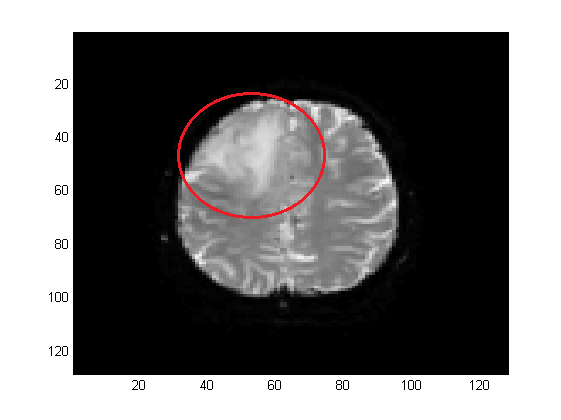
\includegraphics[scale=0.5,angle=0]{ImageGray.png}
    \caption{Area presenting the pathology.}
    \label{fig:CleanGray}
\end{figure}

By applying Algorithm \ref{alg:algorithm1} on the ROI with a number of class $N_{class} = 2$ and $N_{class} = 3$, we get some results which are shown in Figures \ref{fig:Result},\ref{fig:Result2},\ref{fig:Result3}.

\begin{figure}
\centering
    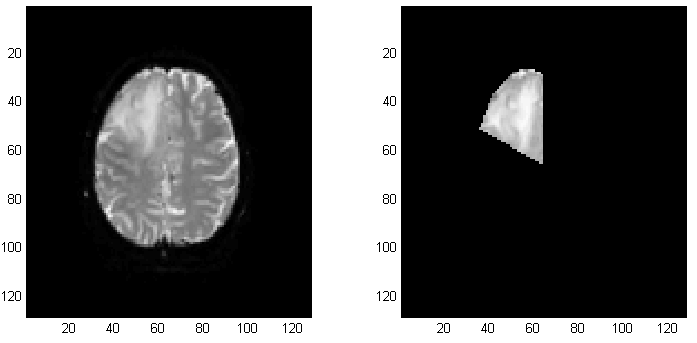
\includegraphics[scale=0.45,angle=0]{Result.png}
    \caption{Results of the algorithm. left: MRI image. right: Mask applied.}
    \label{fig:Result}
\end{figure}

\begin{figure}
\centering
    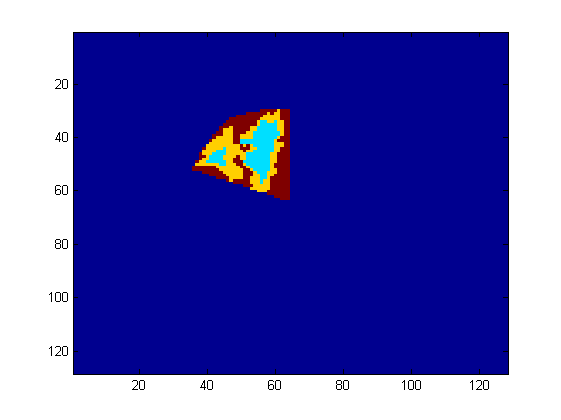
\includegraphics[scale=0.5,angle=0]{3class.png}
    \caption{The results of the algorithm for $N_{class} = 2$.}
    \label{fig:Result2}
\end{figure}

\begin{figure}
\centering
    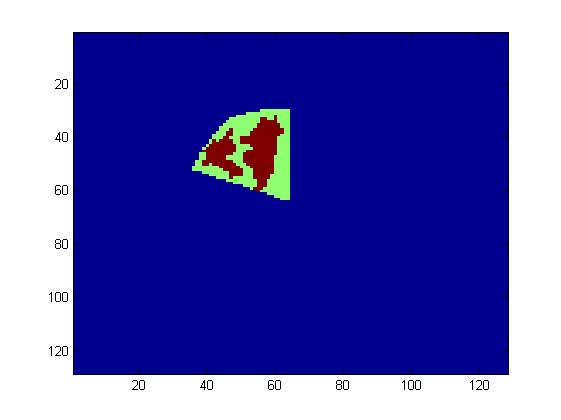
\includegraphics[scale=0.5,angle=0]{2class.png}
    \caption{The results of the algorithm for $N_{class} = 2$.}
    \label{fig:Result3}
\end{figure}

Our experimental results show that the algorithm can easily isolate the pathology from the normal tissues. By adjusting $N_{class} = 3$, we can generate a third class representing the uncertain zone.

\medskip

The results are satisfying. Our similitude matrix depends only on the neighbourhood of each point so our processing tool-chain is highly independent of the input data. Furthermore, the process is fully automated. The user must provide only the number of class and our program deal with the data in order to calculate the truth table.

Nevertheless, when we are trying to apply other algorithms in order to automatically find the optimal number of class \cite{zelnik2004self}, \cite{mouysset2010contributions}, the results aren't satisfying in the case of real data. For now, our only choice is to provide a set of maps with different value of $N_{class}$ and interpret the results, as it has been done with Figure \ref{fig:Result}, \ref{fig:Result2}, \ref{fig:Result3}.

\medskip

The processing tool-chain that have been implemented have been realized in order to have in the end the exact number of cluster $N$ when we apply the k-means algorithm. That means that in some case the algorithm wouldn't arrive to this number of class but we don't allow this situation to happen. It may have a huge impact on the algorithm.

%------------------------------------------------

\section{Conclusion}

By generalising and modifying the method developed in \cite{tartare2014contribution}, this study proposes a new methodology using spectral clustering for the automatic segmentation of MRI images of brain.

The experimental results show that our algorithm is able to isolate the pathology from healthy tissues. Presently, we have only a reliable algorithm that seems to provide good results. However, we are currently studying two options:

\begin{itemize}
\item Realization of parametric map of the area which can provide other information. For brain tissues, the two relevant parameters are the cerebral blood volume (CBV) and the cerebral blood flow (CBF)  \cite{muir2014quantitative}.
\item Later on, we should realize a multi-modal analyse which imply to analyse other kind of MRI sequences in order to extract other sources of information.

\end{itemize}

We are targeting to provide a unsupervised clustering algorithm which would be able to fully identify and segmented pathological tissues of the brain.


 

%----------------------------------------------------------------------------------------
%	REFERENCE LIST
%----------------------------------------------------------------------------------------


\nocite{*}
\bibliographystyle{IEEEtran}{\small}
\bibliography{IEEEabrv,bibliographie}

%----------------------------------------------------------------------------------------

\end{document}
